% 
% Annual Cognitive Science Conference
% Sample LaTeX Paper -- Proceedings Format
% 

% Original : Ashwin Ram (ashwin@cc.gatech.edu)       04/01/1994
% Modified : Johanna Moore (jmoore@cs.pitt.edu)      03/17/1995
% Modified : David Noelle (noelle@ucsd.edu)          03/15/1996
% Modified : Pat Langley (langley@cs.stanford.edu)   01/26/1997
% Latex2e corrections by Ramin Charles Nakisa        01/28/1997 
% Modified : Tina Eliassi-Rad (eliassi@cs.wisc.edu)  01/31/1998
% Modified : Trisha Yannuzzi (trisha@ircs.upenn.edu) 12/28/1999 (in process)
% Modified : Mary Ellen Foster (M.E.Foster@ed.ac.uk) 12/11/2000
% Modified : Ken Forbus                              01/23/2004
% Modified : Eli M. Silk (esilk@pitt.edu)            05/24/2005
% Modified : Niels Taatgen (taatgen@cmu.edu)         10/24/2006
% Modified : David Noelle (dnoelle@ucmerced.edu)     11/19/2014
% Modified : Roger Levy (rplevy@mit.edu)     12/31/2018



%% Change "letterpaper" in the following line to "a4paper" if you must.

\documentclass[10pt,letterpaper]{article}

\usepackage{cogsci}
\usepackage{color}
\usepackage{graphicx}

%\cogscifinalcopy % Uncomment this line for the final submission 

\usepackage{pslatex}
\usepackage{apacite}
\usepackage{float} % Roger Levy added this and changed figure/table
                   % placement to [H] for conformity to Word template,
                   % though floating tables and figures to top is
                   % still generally recommended!

%\usepackage[none]{hyphenat} % Sometimes it can be useful to turn off
%hyphenation for purposes such as spell checking of the resulting
%PDF.  Uncomment this block to turn off hyphenation.

\definecolor{Orange}{RGB}{255,140,0}
\newcommand{\ek}[1]{\textcolor{Orange}{[ek: #1]}} 

%\setlength\titlebox{4.5cm}
% You can expand the titlebox if you need extra space
% to show all the authors. Please do not make the titlebox
% smaller than 4.5cm (the original size).
%%If you do, we reserve the right to require you to change it back in
%%the camera-ready version, which could interfere with the timely
%%appearance of your paper in the Proceedings.



\title{How to Make a Proceedings Paper Submission}
 
\author{{\large \bf Morton Ann Gernsbacher (MAG@Macc.Wisc.Edu)} \\
  Department of Psychology, 1202 W. Johnson Street \\
  Madison, WI 53706 USA
  \AND {\large \bf Sharon J.~Derry (SDJ@Macc.Wisc.Edu)} \\
  Department of Educational Psychology, 1025 W. Johnson Street \\
  Madison, WI 53706 USA}


\begin{document}

\maketitle


\begin{abstract}
Include no author information in the initial submission, to facilitate
blind review.  The abstract should be one paragraph, indented 1/8~inch on both sides,
in 9~point font with single spacing. The heading ``{\bf Abstract}''
should be 10~point, bold, centered, with one line of space below
it. This one-paragraph abstract section is required only for standard
six page proceedings papers. Following the abstract should be a blank
line, followed by the header ``{\bf Keywords:}'' and a list of
descriptive keywords separated by semicolons, all in 9~point font, as
shown below.

\textbf{Keywords:} 
add your choice of indexing terms or keywords; kindly use a
semicolon; between each term
\end{abstract}

\section{Introduction}
\ek{make up your mind about generations vs. reproduction; original stories vs. seeds; stories vs. storytype vs. condition,...}

%\begin{figure}[H]
%	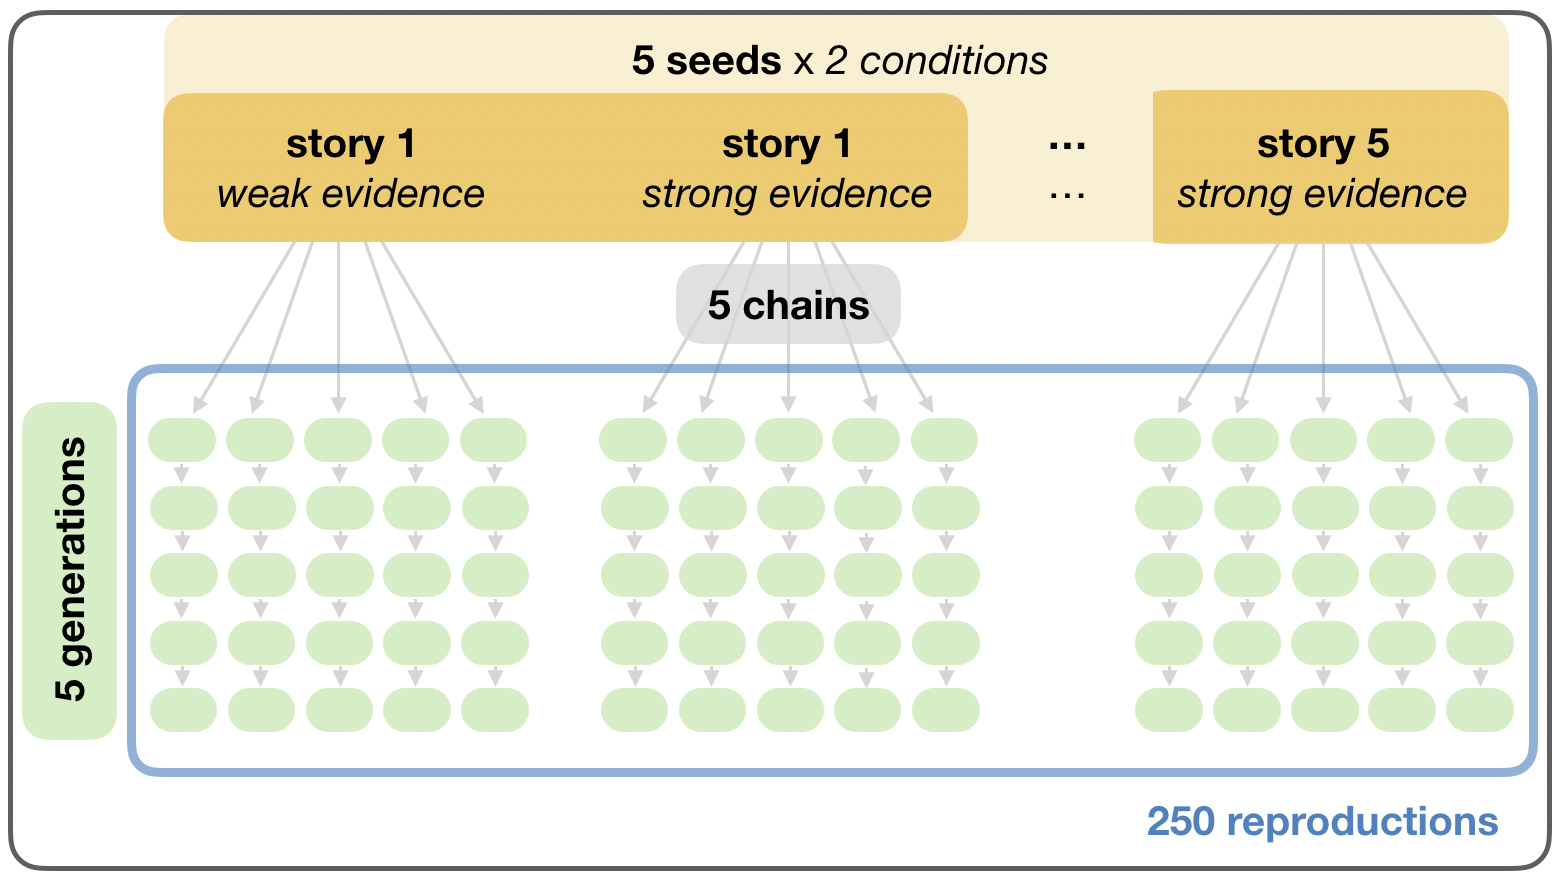
\includegraphics[width=0.48\textwidth]{graphs/corpus_overview.png}
%	\caption{This is a figure.} 
%	\label{overview-figure}
%\end{figure}

\section{Corpus Collection}
\ek{transmission chain method}

\subsection{Material}
We constructed five crime stories which stand in the beginning of each reproduction chain. These will be referred to as seeds. All of these stories share a \ek{news-article-tone} and follow a similar reporting structure: They report a crime that has happened, the police's search for the people who committed the crime, the arrest of one or multiple suspects and the possible punishment they face if found guilty. Furthermore, each of these five seed stories can occur in either of two conditions: a weak evidence or strong evidence condition. This manipulation was achieved by varying the final sentence of the story.

\subsection{Methods}
74 Stanford students participated in this online study as part of their course requirements \ek{include \_babe reference?}. Each participant read and reproduced each of the five stories with a random condition. After reading the instructions, participants read the story and whenever ready could proceed to the free reproduction and the story disappeared. The trial order was randomized.\\
A complete chain is a chain that has 5 reproductions/generations. For our subsequent analyses, we randomly chose 50 complete chains, evenly distributed of stories and conditions. Overall, this gives us a corpus that comprises 250 reproductions and 10 original stories.

\subsection{Results}

%\begin{figure}[H]
%	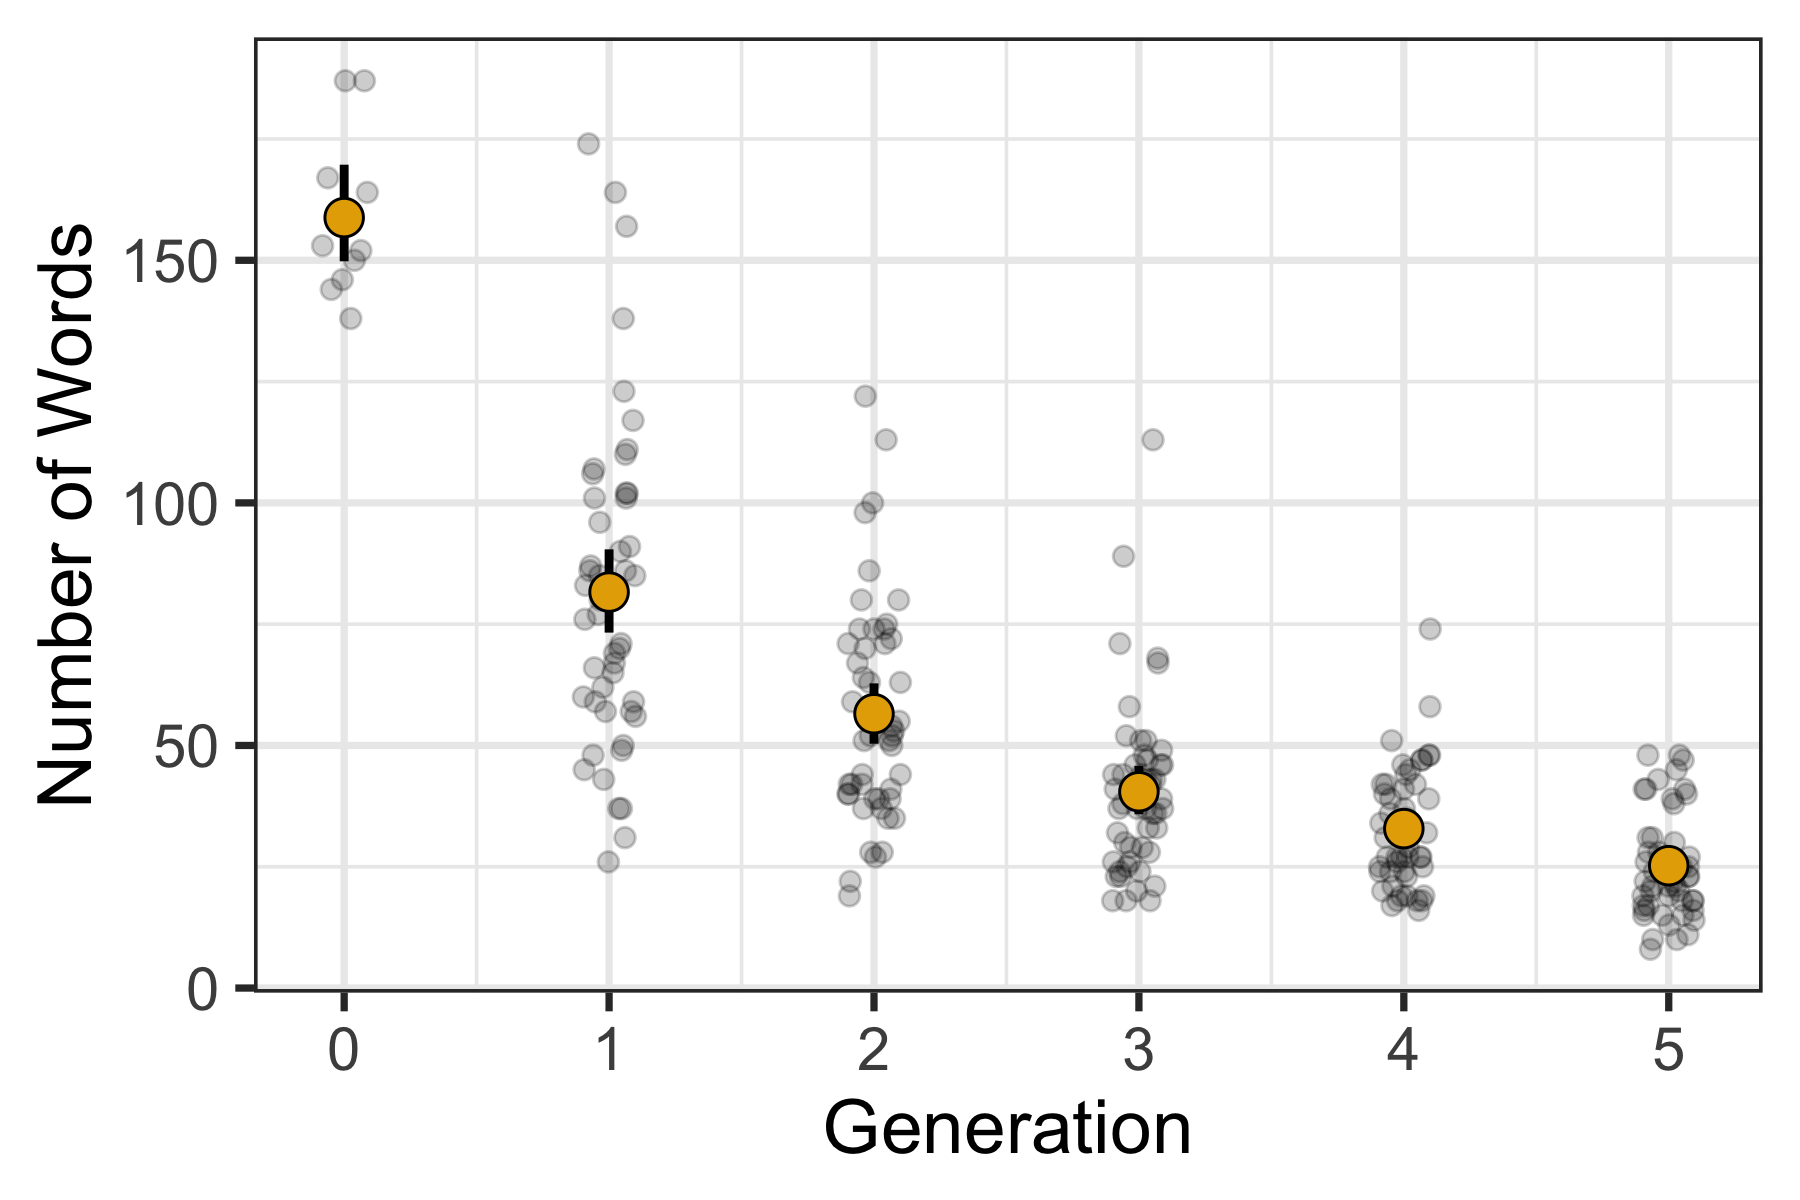
\includegraphics[width=0.48\textwidth]{graphs/corpus_length.png}
%	\caption{This is a figure.} 
%	\label{sample-figure}
%\end{figure}

As expected (\ek{cite!}), the length of reproductions decreases on average with the highest decrease in the first 3 generations. The difference between the fourth and fifth generation turns almost negligible which could be a sign for an almost perfect recall at this length (\ek{cite}).

\section{Subjective Ratings}
To evaluate the reproduction corpus, we would like to trace a variety of psychological variables trough stories and generations. To obtain these, we conducted an Amazon Mechanical Turk study asking questions about the suspect, the author, the reader and the evidence.

\subsection{Material}
The stories were taken from the corpus described in \ek{ref}.\\
In the questions, we asked about the evidence, the suspect's guilt and possible conviction, the reader's beliefs about the author and the reader's emotional connection to the story. \ek{a complete list of the questions can be found...} Overall, participants were asked eight questions of interest and four attention check questions. 

\subsection{Methods}
\ek{number of participants} participants were recruited over Amazon Mechanical Turk. Each participant read one story and answered twelve questions (including four attention check questions). They indicate their response by moving a slider on a continuous scale \ek{Doesn't apply button?}. Each question was shown in isolation in a randomized order. The story was visible at all times.


\subsection{Results}

\section{Conclusion}

\section{Discussion}

%
%
%\section{General Formatting Instructions}
%
%The entire content of a paper (including figures, references, and anything else) can be no longer than six pages in the \textbf{initial submission}. In the \textbf{final submission}, the text of the paper, including an author line, must fit on six pages. Up to one additional page can be used for acknowledgements and references.
%
%The text of the paper should be formatted in two columns with an
%overall width of 7 inches (17.8 cm) and length of 9.25 inches (23.5
%cm), with 0.25 inches between the columns. Leave two line spaces
%between the last author listed and the text of the paper; the text of
%the paper (starting with the abstract) should begin no less than 2.75 inches below the top of the
%page. The left margin should be 0.75 inches and the top margin should
%be 1 inch.  \textbf{The right and bottom margins will depend on
%  whether you use U.S. letter or A4 paper, so you must be sure to
%  measure the width of the printed text.} Use 10~point Times Roman
%with 12~point vertical spacing, unless otherwise specified.
%
%The title should be in 14~point bold font, centered. The title should
%be formatted with initial caps (the first letter of content words
%capitalized and the rest lower case). In the initial submission, the
%phrase ``Anonymous CogSci submission'' should appear below the title,
%centered, in 11~point bold font.  In the final submission, each
%author's name should appear on a separate line, 11~point bold, and
%centered, with the author's email address in parentheses. Under each
%author's name list the author's affiliation and postal address in
%ordinary 10~point type.
%
%Indent the first line of each paragraph by 1/8~inch (except for the
%first paragraph of a new section). Do not add extra vertical space
%between paragraphs.
%
%
%\section{First Level Headings}
%
%First level headings should be in 12~point, initial caps, bold and
%centered. Leave one line space above the heading and 1/4~line space
%below the heading.
%
%
%\subsection{Second Level Headings}
%
%Second level headings should be 11~point, initial caps, bold, and
%flush left. Leave one line space above the heading and 1/4~line
%space below the heading.
%
%
%\subsubsection{Third Level Headings}
%
%Third level headings should be 10~point, initial caps, bold, and flush
%left. Leave one line space above the heading, but no space after the
%heading.
%
%
%\section{Formalities, Footnotes, and Floats}
%
%Use standard APA citation format. Citations within the text should
%include the author's last name and year. If the authors' names are
%included in the sentence, place only the year in parentheses, as in
%\citeA{NewellSimon1972a}, but otherwise place the entire reference in
%parentheses with the authors and year separated by a comma
%\cite{NewellSimon1972a}. List multiple references alphabetically and
%separate them by semicolons
%\cite{ChalnickBillman1988a,NewellSimon1972a}. Use the
%``et~al.'' construction only after listing all the authors to a
%publication in an earlier reference and for citations with four or
%more authors.
%
%
%\subsection{Footnotes}
%
%Indicate footnotes with a number\footnote{Sample of the first
%footnote.} in the text. Place the footnotes in 9~point font at the
%bottom of the column on which they appear. Precede the footnote block
%with a horizontal rule.\footnote{Sample of the second footnote.}
%
%
%\subsection{Tables}
%
%Number tables consecutively. Place the table number and title (in
%10~point) above the table with one line space above the caption and
%one line space below it, as in Table~\ref{sample-table}. You may float
%tables to the top or bottom of a column, and you may set wide tables across
%both columns.
%
%\begin{table}[H]
%\begin{center} 
%\caption{Sample table title.} 
%\label{sample-table} 
%\vskip 0.12in
%\begin{tabular}{ll} 
%\hline
%Error type    &  Example \\
%\hline
%Take smaller        &   63 - 44 = 21 \\
%Always borrow~~~~   &   96 - 42 = 34 \\
%0 - N = N           &   70 - 47 = 37 \\
%0 - N = 0           &   70 - 47 = 30 \\
%\hline
%\end{tabular} 
%\end{center} 
%\end{table}
%
%
%\subsection{Figures}
%
%All artwork must be very dark for purposes of reproduction and should
%not be hand drawn. Number figures sequentially, placing the figure
%number and caption, in 10~point, after the figure with one line space
%above the caption and one line space below it, as in
%Figure~\ref{sample-figure}. If necessary, leave extra white space at
%the bottom of the page to avoid splitting the figure and figure
%caption. You may float figures to the top or bottom of a column, and
%you may set wide figures across both columns.
%
%\begin{figure}[H]
%\begin{center}
%\fbox{CoGNiTiVe ScIeNcE}
%\end{center}
%\caption{This is a figure.} 
%\label{sample-figure}
%\end{figure}
%
%
%\section{Acknowledgments}
%
%In the \textbf{initial submission}, please \textbf{do not include
%  acknowledgements}, to preserve anonymity.  In the \textbf{final submission},
%place acknowledgments (including funding information) in a section \textbf{at
%the end of the paper}.
%
%
%\section{References Instructions}
%
%Follow the APA Publication Manual for citation format, both within the
%text and in the reference list, with the following exceptions: (a) do
%not cite the page numbers of any book, including chapters in edited
%volumes; (b) use the same format for unpublished references as for
%published ones. Alphabetize references by the surnames of the authors,
%with single author entries preceding multiple author entries. Order
%references by the same authors by the year of publication, with the
%earliest first.
%
%Use a first level section heading, ``{\bf References}'', as shown
%below. Use a hanging indent style, with the first line of the
%reference flush against the left margin and subsequent lines indented
%by 1/8~inch. Below are example references for a conference paper, book
%chapter, journal article, dissertation, book, technical report, and
%edited volume, respectively.
%
%\nocite{ChalnickBillman1988a}
%\nocite{Feigenbaum1963a}
%\nocite{Hill1983a}
%\nocite{OhlssonLangley1985a}
%% \nocite{Lewis1978a}
%\nocite{Matlock2001}
%\nocite{NewellSimon1972a}
%\nocite{ShragerLangley1990a}


\bibliographystyle{apacite}

\setlength{\bibleftmargin}{.125in}
\setlength{\bibindent}{-\bibleftmargin}

\bibliography{CogSci_Template}


\end{document}
